\section*{Question 1}
\fakesection{1}

This problem compares separately filtering then downsampling a signal, versus applying a polyphase decimator. The input signal contains four tones: 50, 150, 950 and 1050 Hz.

\begin{figure}[ht]
    \centering
    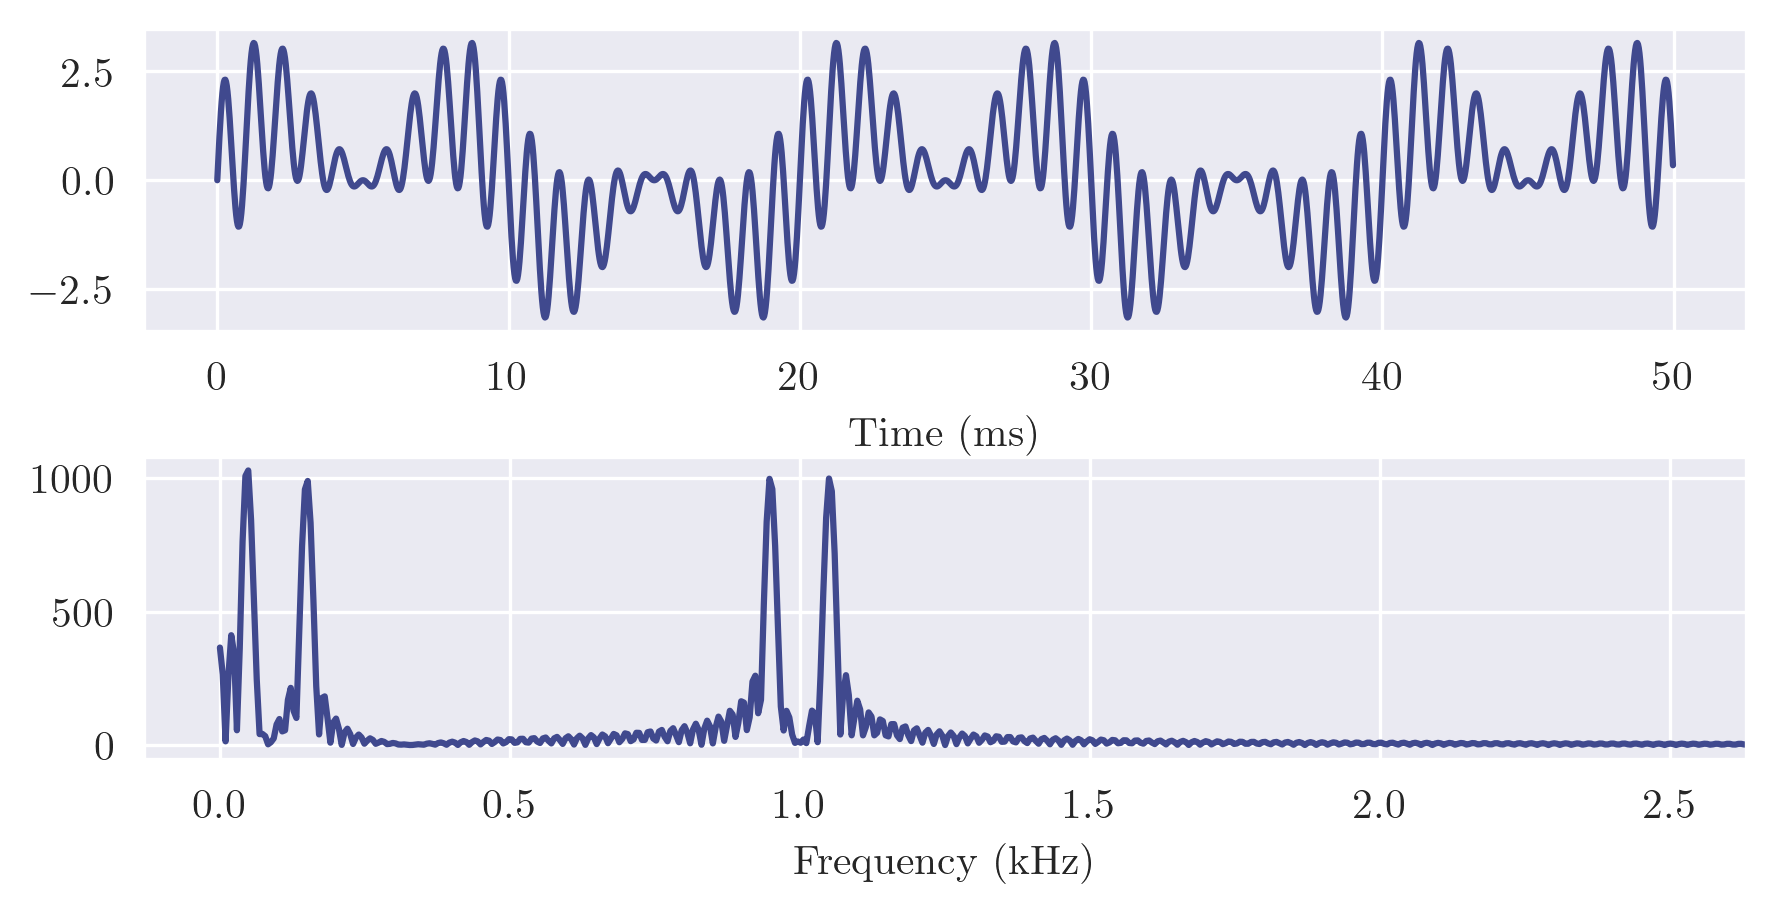
\includegraphics[width=0.8\textwidth]{images/q1_signal.png}
    \caption{Input signal contains tones at 50, 150, 950 and 1050 Hz}
    \label{fig:q1_signal}
\end{figure}

We first investigate separately filtering then downsampling the signal. The signal is sampled at 40 kHz. We are interested in retaining only the tones at 50 and 150 Hz; therefore, we apply a Kaiser-windowed LPF with a pass band up to 200 Hz and transition band of 100 Hz. Comparing the pass and stop band attenuation requirements, 3 dB and 100 dB down, respectively, we find the necessary attentuation is $A=100dB$. The filter length can then be estimated at:
\begin{align}
    N = \frac{A - 7.96}{14.36(\Delta f/f_s)} \approx 2564.07
\end{align}
which we choose to round up to 2566. We can now formulate a Kaiser window:
\begin{align}
    w(n) = \frac{I_0(\beta(1 - [2n/(N-1)]^2)^{1/2})}{I_0(\beta)},\ |n| \leq (N-1)/2
\end{align}
where $I_0$ is the Bessel function of the first kind and $\beta$ is a piecewise function of the required attenuation, $A$ (dB):
\begin{align}
    \beta = \begin{cases}
        0,                                      & A \leq 21 \\
        0.5842(A - 21)^{0.4} + 0.07886(A - 21), & 21 < A \leq 50 \\
        0.1102(A - 8.7),                        & A \geq 50
    \end{cases}
\end{align}
Hence, our value of $\beta$ for $A=100$ dB is:
\begin{align}
    \beta = 0.1102(100 - 8.7) \approx 10.06126
\end{align}
We now create the ideal frequency response vector, with a number of bins in the pass band given by
\begin{align}
    N \cdot \frac{f_s/2 - f_p}{f_s} = 12.83 \approx 13
\end{align}
Applying the Kaiser window to the ideal filter then convolving with the input signal, we obtain the filtered signal of Figure \ref{fig:q1_filt}.

\begin{figure}[ht]
    \centering
    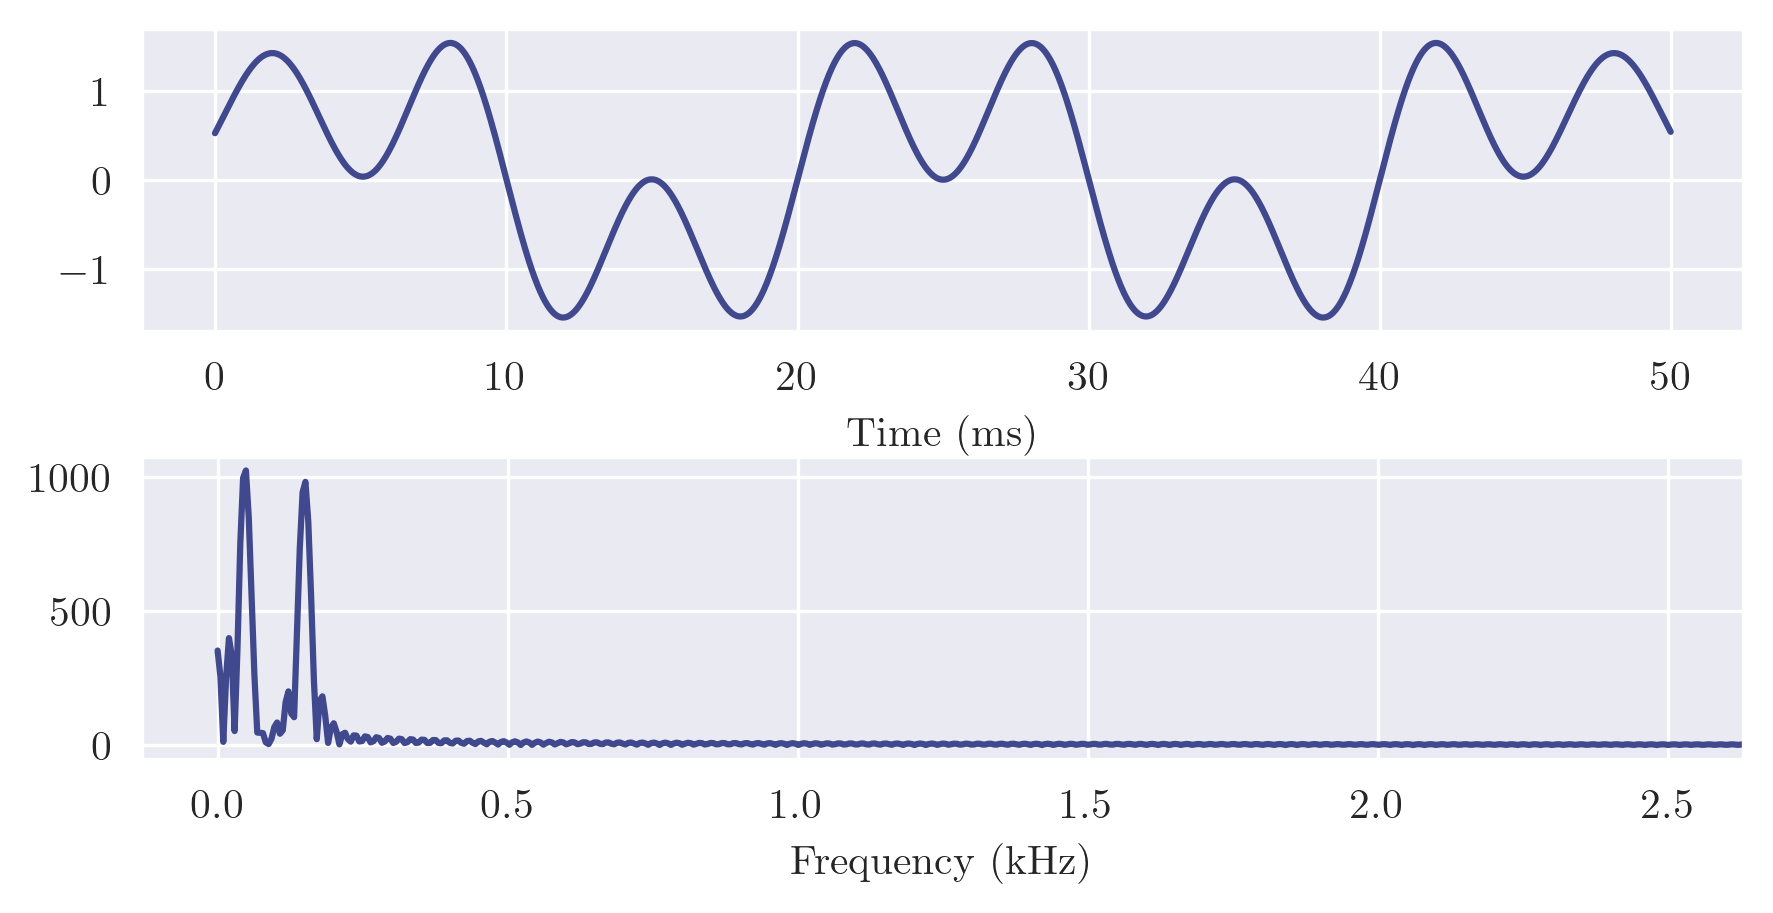
\includegraphics[width=0.8\textwidth]{images/q1_filt.png}
    \caption{Filtered signal containing only tones at 50 and 150 Hz}
    \label{fig:q1_filt}
\end{figure}

Finally, we maximally downsample by a factor of $M$, given by
\begin{align}
    M = \frac{f_s}{f_{BW} + \Delta f} = 80
\end{align}
where $f_{BW}$ is the bandwidth, equal to twice the pass band width. We downsample by selecting every $M$th element in the signal and discarding the others, obtaining the following result.

\begin{figure}[ht]
    \centering
    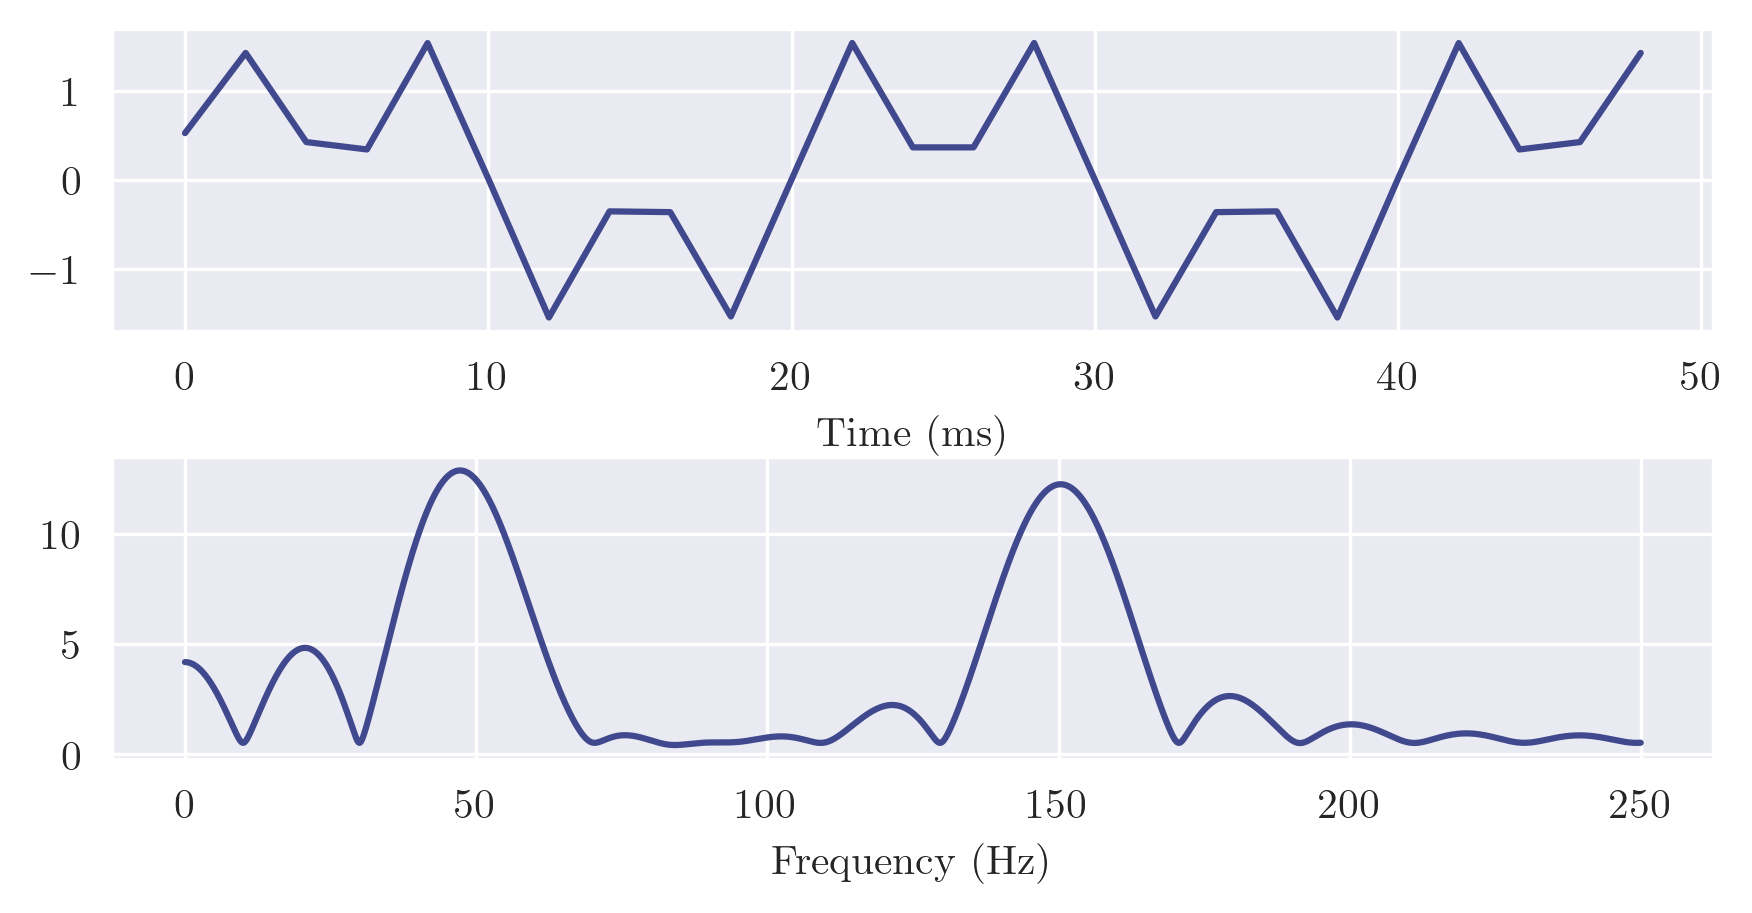
\includegraphics[width=0.8\textwidth]{images/q1_dsamp.png}
    \caption{Filtered signal maximally downsampled by a factor of $M$=80}
    \label{fig:q1_dsamp}
\end{figure}

\newpage

We now investigate repeating the filtering and downsampling using a polyphase decimator. We zero-pad both the Kaiser-windowed LPF coefficients and the input signal to a multiple of $M$, then reshape both into column-major matrices with $M$ rows. Each row of filter coefficients is convolved with its corresponding row of the input signal, and the resulting $M$ outputs are element-wise summed. After removing transient edge effects, the overall output signal is therefore a factor of $M$ shorter than the input signal.

\begin{figure}[ht]
    \centering
    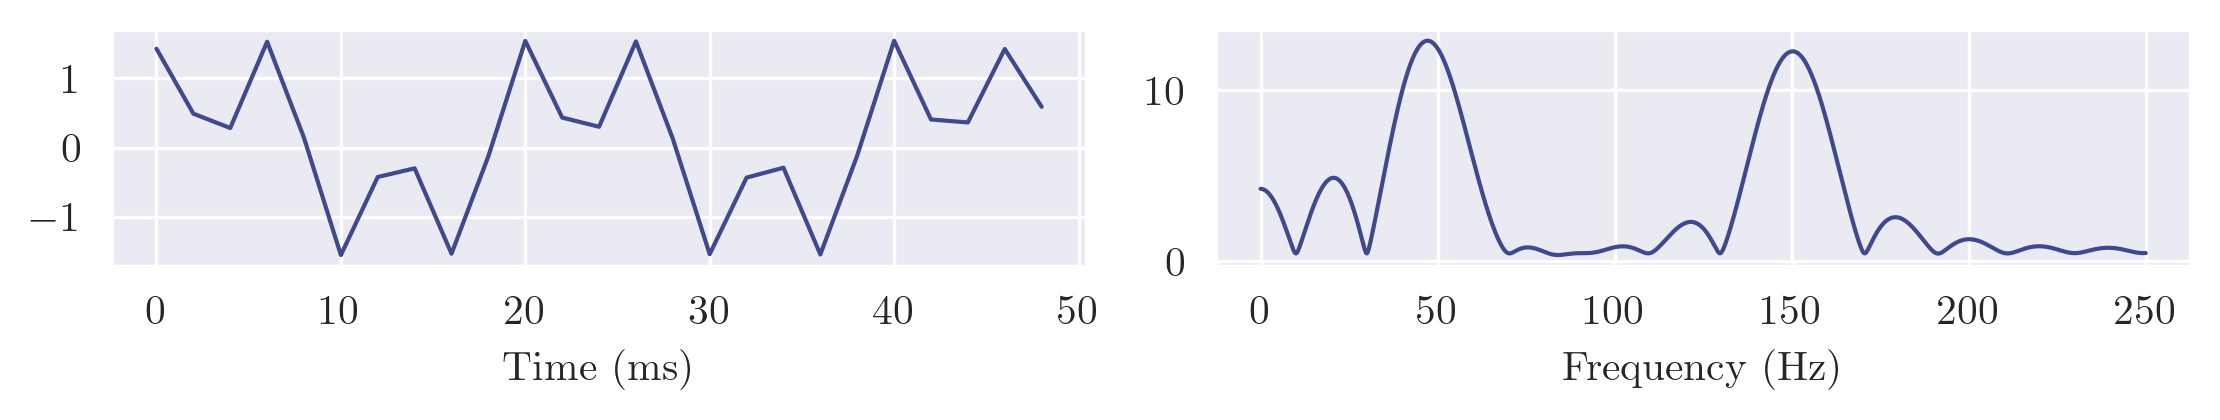
\includegraphics[width=0.8\textwidth]{images/q1_polydecimate.png}
    \caption{Polyphase decimator applied to input signal, achieving filtering and downsampling}
    \label{fig:q1_polydecimate}
\end{figure}

Observe that the polyphase decimator produces the same result as separately filtering then downsampling. However, per the first noble identity, the polyphase decimator requires a factor of $M$ less computations to achieve the same result. Intuitively, by filtering then downsampling by a factor of $M$, $M-1$ of the filtered results are immediately discarded. By filtering after downsampling, the polyphase decimator achieves a theoretical $M$-fold performance gain.

We can test this theory by timing repeated trials of either method as a proxy for the number of computations. Using 10,000 trials, we find the following average times:
\begin{itemize}
    \item Filter then downsample: 1.327 ms
    \item Polyphase decimator: 0.831 ms
\end{itemize}
While the polyphase method is undoubtedly faster, unlike the theory suggests, we find only a 40\% speedup compared to the naive method. Initially, it was speculated that caching may have skewed the results; however, this was disproven by randomising the signals for each trial and observing no change in timings. Overhead was the next most likely reason and was tested by increasing the sampling rate of the input signal to 40 MHz. However, the polyphase method then took 60\% \textit{longer} than the naive method. This strongly suggests that the polyphase method has a larger overhead than the naive method. This is no doubt implementation specific and kernel optimisations are out of the scope of this problem. In all likelihood, \texttt{scipy}'s convolution is excruciatingly optimised, and by splitting the convolution some of that optimisation potential is lost while adding more overhead.
